\section{Capacit\`a di Canale} \label{sec:can}
Si considera ora il caso di una trasmissione in cui sia presente un canale non ideale, ovvero in cui \textit{non è certo che quello che viene inviato corrisponda a quello che viene ricevuto}. Il problema che ci poniamo è quindi l’\textbf{affidabilità} della trasmissione: la codifica di canale affronta il problema di trasmettere in maniera affidabile su un canale non affidabile. La codifica di canale è strettamente collegata alla capacit\`a di canale, ovvero alla capacità del canale di “far passare” l’informazione, che, come vedremo, ci porter\`a al Secondo Teorema di Shannon. Codifica di canale e di sorgente sono duali ma separate:
\begin{itemize}
    \item Con la codifica di sorgente si toglie la ridondanza per comprimere l’informazione.
    \item Con la codifica di canale si vuole aumentare l’affidabilità della trasmissione aggiungendo ridondanza al segnale trasmesso: si cerca un compromesso tra affidabilità ed efficienza realizzando un processo di codifica a controllo d’errore per ridurre gli effetti del rumore presente sul canale.
\end{itemize}
\subsection{Canale}
Il concetto di canale è piuttosto ampio: rappresenta ciò che succede ad un’informazione tra sorgente e
destinatario. Può includere, a seconda delle necessità, solo il mezzo fisico (ad esempio il solo doppino telefonico o un nastro magnetico) o, ad esempio, anche tutto ciò che è compreso tra un microfono e un altoparlante. Alcuni esempi di canale possono essere
\begin{itemize}
    \item Linea telefonica /ADSL (rumore termico, distorsioni, cross-talk, ...).
    \item Comunicazioni wireless (attenuazione atmosfera, rumore termico, interferenze, ...).
    \item Hard-disk\footnote{Non necessariamente la comunicazione deve avvenire tra due oggetti distinti, si pu\`o pensare che la sorgente e il destinatario siano lo stesso oggetto ma a tempi differenti, come nel caso della memorizzazione dell'informazione.} (errori di lettura/scrittura, materiali imperfetti, ...).
\end{itemize}
In ogni caso, in un canale, esiste \textit{sempre} la presenza di rumore che compromette la trasmissione.
\subsubsection{Canale discreto senza memoria}
\defn{\textit{Canale discreto senza memoria tempo-invariante:}} Si definisce canale discreto senza memoria tempo-invariante un canale in cui:
\begin{itemize}
    \item I simboli in uscita dalla sorgente (quindi in ingresso al canale) e in uscita dal canale, appartengano ad un alfabeto finito.
    \item In uscita dal canale si ha una sequenza che è casuale ma ha una distribuzione statistica che dipende dalla sequenza in ingresso.
    \item L’uscita in un determinato istante dipende solo dal simbolo in ingresso al canale in quell’istante e non
dai simboli precedentemente trasmessi.
    \item Le proprietà del canale non variano nel tempo.
\end{itemize}
Un canale discreto senza memoria tempo-invariante è univocamente definito dall’alfabeto di ingresso $A$, l'alfabeto di uscita $B$ e le \textit{forward probability} $p(b|a)$.
\begin{figure}[H]
    \centering
    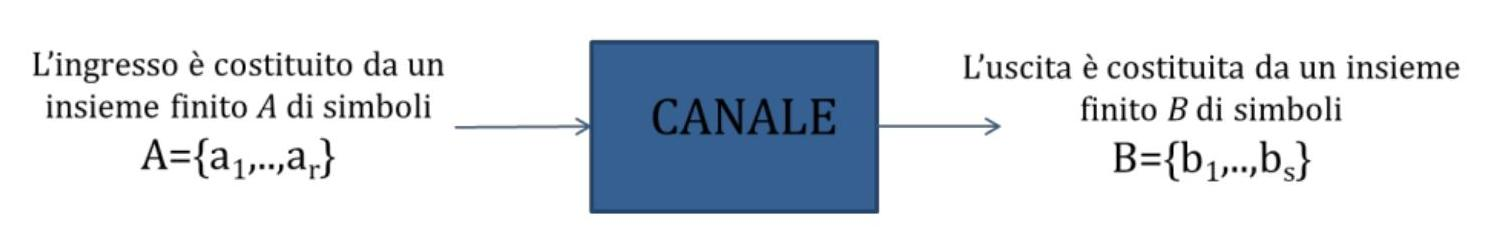
\includegraphics[width=\textwidth]{img/canale.jpg}
    \caption{Schema ad alto livello di un canale di comunicazione.}
    \label{fig:canale}
\end{figure}
In ricezione, dalla sequenza in uscita, si prova a ricostruire la sequenza di ingresso. Siccome per\`o due o più
input possono portare alla stessa parola in uscita dal canale, la ricostruzione della sequenza originaria può
essere \textbf{affetta da errori}: la comunicazione ha successo quando il ricevitore ed il trasmettitore \textit{concordano} su ciò che è stato trasmesso. Un canale può essere rappresentato con un grafo o, equivalentemente, con una matrice di canale $\mathcal{P}$

\begin{mybox}{green}{\textit{\textbf{Esempio 1} : \textbf{Rappresentazioni di canale}}}
Detto $X=\{x_1, x_2\}$ l'alfabeto d'ingresso e $Y = \{y_1, y_2, y_3\}$ l'alfabeto di uscita si hanno le seguenti rappresentazioni equivalenti

\begin{minipage}{0.45\textwidth}
\begin{figure}[H]
    \centering
    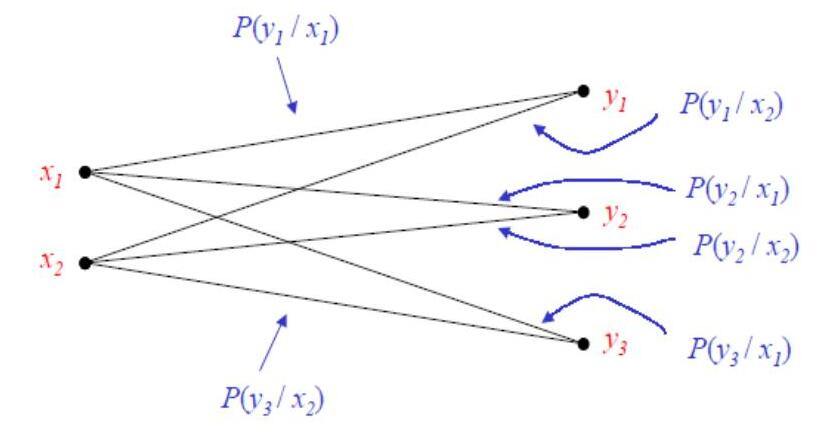
\includegraphics[scale=0.2]{img/grafo.jpg}
    \caption{Rappresentazione a grafo di un canale.}
\end{figure}
\end{minipage}
\begin{minipage}{0.45\textwidth}
\begin{equation*}
    \mathcal{P} = \begin{bmatrix}
    p(y_1|x_1) & p(y_2|x_1) & p(y_3|x_1) \\
    p(y_1|x_2) & p(y_2|x_2) & p(y_3|x_2) \\
    \end{bmatrix}
\end{equation*}
\end{minipage}
\end{mybox}
in cui si ha che le $\mathcal{P}_{ij} = p(b_j|a_i)$ e che le righe sommano ad $1$\footnote{Questo serve a garantire che per ogni input $a$ verr\`a effettivamente generato un output.}: $\sum_{j=1}^s p(b_j|a_i) = 1, \forall i=1,\dots,r$. \\
Se in ingresso al canale invece dei singoli elementi dell’alfabeto abbiamo sequenze di $n$ simboli dobbiamo fare riferimento all'estensione $n$-esima della sorgente $A^n$ e del destinatario $B^n$. Il canale in questo caso \`e completamente definito dai due alfabeti $A^n, B^n$ e dalla matrice di canale $\Pi$ data dal prodotto di Kronecker $n$ volte della matrice $\mathcal{P}$ del canale originario:
\begin{equation}
    \Pi = \underbrace{\mathcal{P} \otimes \mathcal{P} \otimes \dots \otimes \mathcal{P}}_n
\end{equation}
\\
Chiariamo la \textbf{notazione}:
\begin{itemize}
    \item $p(a)$ rappresenta la probabilit\`a \textbf{a priori} dei simboli in ingresso, ovvero la probabilit\`a che la sorgente emetta il simbolo $a$.
    \item $p(b)$ rappresenta la probabilità che a destinazione venga ricevuto il simbolo $b$.
    \item $p(a,b)$ rappresenta la probabilità congiunta che sia stato trasmesso il simbolo $a$ e che venga ricevuto il simbolo $b$.
    \item $p(b|a)$ rappresenta la probabilità condizionata che sia stato ricevuto il simbolo $b$ dato che è stato trasmesso il simbolo $a$, \`e quella che abbiamo definito \textbf{forward probability}.
    \item $p(a|b)$ rappresenta la probabilità condizionata che sia stato trasmesso il simbolo $a$ dato che è stato ricevuto il simbolo $b$, prende il nome di \textbf{backward probability}, ed \`e la probabilit\`a \textbf{a posteriori} dei simboli in ingresso.
\end{itemize}
Si possono quindi definire due entropie: l'entropia \textit{a priori}
\begin{equation}
    H(A) = \sum_{a \in A} p(a) \log \info{a}
\end{equation}
e l'entropia \textit{a posteriori}
\begin{equation}
    H(A|b) = \sum_{a \in A} p(a,b) \log \frac{1}{p(a|b)}
\end{equation}
che, come abbiamo detto, rappresentano il numero medio di cifre binarie necessarie per rappresentare $A$, rispettivamente considerando solo la sorgente e considerando di poter osservare la particolare uscita $b$ del canale. \\
Mediando su tutti i possibili simboli ricevuti
\begin{equation}
    H(A|B) = \sum_{b \in B} H(A|b) = \sum_{b \in A} \sum_{a \in A} p(a,b) \log \frac{1}{p(a|b)}
\end{equation}
si ha l’informazione media sulla sorgente conoscendo
i simboli ricevuti, ovvero l’incertezza rimasta su $A$ dopo aver conosciuto $B$. Questa quantit\`a prende il nome di \textbf{equivocazione di canale} e rappresenta l’informazione aggiuntiva che serve in ricezione dopo aver osservato $B$, quindi \textbf{ci\`o che si \`e perso a causa del canale}.\\
Se ci mettiamo dalla parte del destinatario al tempo $0$ non abbiamo visto arrivare alcun simbolo dal
canale e la nostra “incertezza” sulla sorgente $A$ è pertanto l’entropia $H(A)$. Dopo l'osservazione però, la nostra incertezza si riduce a $H(A|B)$. L'informazione che ha viaggiato sul canale \`e dunque
\begin{equation}
    H(A) - H(A|B) = I(A;B) = \sum_{a \in A} \sum_{b \in B} p(a,b) \frac{p(a,b)}{p(a)p(b)}
\end{equation}
Infatti, ricordando che $I(A;B)$ è l’informazione contenuta sia in $A$ che in $B$, si ha che questa rappresenta ciò che effettivamente ha attraversato il canale. Di conseguenza la \textit{massima quantità di informazione che può viaggiare attraverso un canale è data dal massimo valore che può assumere l’informazione mutua}.

\subsubsection{Capacit\`a di Canale}
Abbiamo detto quindi che la massima quantità di informazione che può viaggiare attraverso un canale è quindi data dal massimo valore che può assumere l'informazione mutua. Questa per\`o dipende sia dalla probabilit\`a a priori $p(a)$ che dalla forward probability $p(b|a)$ quindi, rispettivamente, dalla sorgente e dalla matrice di canale. Infatti quanta informazione arriva a destinazione dipende sia dal tipo di canale considerato che anche dall’uso che viene fatto del canale. Se vogliamo massimizzare l’informazione trasportata dal canale dobbiamo anche agire sulla sorgente. \\
Al fine di caratterizzare un canale discreto senza memoria \textbf{indipendentemente dalla sorgente in ingresso}, si definisce capacità del canale il valore massimo dell’informazione mutua rispetto a tutte le possibili distribuzioni delle probabilità dei simboli di ingresso:
\defn{\textit{Capacit\`a di Canale:}} Misurata in $[bit/simbolo]$ la capacit\`a di canale $\mathcal{C}$ \`e  definita come
\begin{equation}
    \mathcal{C} \coloneqq \max_{p(a)} I(A;B)
\end{equation}
Se si massimizza su $p(a)$, $\mathcal{C}$ dipende solo dal canale stesso e \textit{rappresenta il massimo flusso informativo che può essere sopportato dal canale}. Se, inoltre, la sorgente genera simboli con una frequenza $f$ ($[simboli/s]$) la capacit\`a di canale per unit\`a di tempo \`e data da
\begin{equation}
    \mathcal{C}_t \coloneqq f \mathcal{C}, \hspace{15pt} [bit/s]
\end{equation}
La capacità di canale per unità di tempo $\mathcal{C}_t$ rappresenta la \textit{massima velocità di trasferimento dell’informazione permessa dal canale}. Si hanno alcune propriet\`a per la capacit\` di canale:
\begin{itemize}
    \item $\mathcal{C} \geq 0$
    \item $\mathcal{C} \leq \log |A|$ (dato che $I(A;B) \leq H(A) \leq \log |A|$)
    \item $\mathcal{C} \leq \log |B|$ (dato che $I(A;B) \leq H(B) \leq \log |B|$)
    \item $I(A;B)$ \`e una funzione continua di $p(a)$
    \item $I(A;B)$ \`e una funzione concava di $p(a)$, per cui si ha coincidenza tra massimi locali e massimi globali.
\end{itemize}
Per determinare la capacità si deve quindi effettuare una massimizzazione. Si possono quindi usare tecniche di ottimizzazione, anche se in generale non è semplice. Ci sono per\`o dei casi particolari in cui la capacità può essere calcolata senza troppi sforzi, vediamone alcuni.
\subsubsection{Canale senza rumore}
Un canale si definisce \textbf{senza rumore} (noiseless) se è caratterizzato da una matrice di canale $\mathcal{P}$ con $1$ solo elemento non
nullo in ogni colonna. In questo tipo di canale quindi il destinatario sa sempre che simbolo \`e stato inviato mentre il mittente non è in grado di sapere cosa il destinatario abbia ricevuto. Ricordando che $\mathcal{P}$ \`e data da
\begin{equation}
    \mathcal{P} = \begin{bmatrix}
    p(b_1|a_1) & p(b_2|a_1) & \dots & p(b_s|a_1) \\
    p(b_1|a_2) & p(b_2|a_2) & \dots & p(b_s|a_2) \\
    \vdots & \vdots & & \vdots \\
     p(b_1|a_r) & p(b_2|a_r) & \dots & p(b_s|a_r) \\
    \end{bmatrix}
\end{equation}
se un solo elemento per colonna $j$ \`e diverso da $0$ quel simbolo $b_j$ pu\`o essere ottenuto solo con un possibile $a_i$.
Se il canale è noiseless allora $H(A|B) = 0$, ovvero l’equivocazione di canale è nulla, e l'osservazione dell’uscita ci restituisce esattamente l’ingresso.
\begin{mybox}{green}{\textit{\textbf{Esempio 2} : \textbf{Canale senza rumore}}}
\begin{minipage}{0.45\textwidth}
\begin{figure}[H]
    \centering
    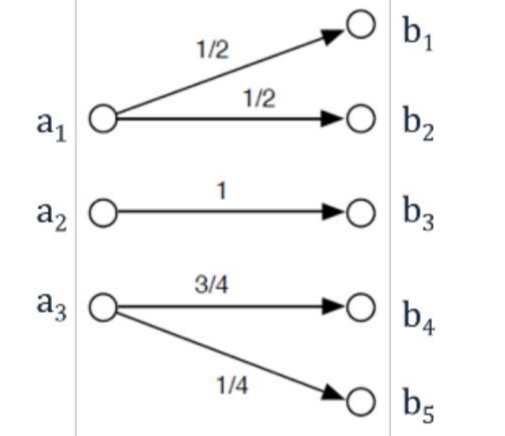
\includegraphics[scale=0.2]{img/detchan.png}
    \caption{Grafo di un canale senza rumore.}
\end{figure}
\end{minipage}
\begin{minipage}{0.45\textwidth}
\begin{equation*}
    \mathcal{P} = \begin{bmatrix}
    1/2 & 1/2 & 0 & 0 & 0 \\
    0 & 0 & 1 & 0 & 0 \\
    0 & 0 & 0 & 3/4 & 1/4
    \end{bmatrix}
\end{equation*}
\end{minipage}
\end{mybox}
Infatti, conoscendo $b$ si determina univocamente $a$ e la probabilit\`a a posteriori \`e data da
\begin{equation*}
    p(a|b) = 
    \begin{cases} 
    1, & \text{se \`e stato trasmesso } a \\
    0, & \text{altrimenti.}
    \end{cases}
\end{equation*}
da cui
\begin{equation*}
    H(A|B) = \sum_{a \in A} \sum_{b \in B} p(a,b) \log \frac{1}{p(a|b)} = 0
\end{equation*}
Si ha quindi che
\begin{equation*}
    I(A;B) = H(A) - H(A|B) = H(A) = \sum_{a \in A} p(a) \info{a}
\end{equation*}
e che, ricordando che l'entropia di una sorgente \`e massima quando i simboli sono tutti equiprobabili\footnote{Cio\`e $p(a) = 1/|A| = 1/r$.} vale 
\begin{equation}
    \mathcal{C} = \max_{p(a)} I(A;B) = \max_{p(a)} \sum_{a \in A} p(a) \info{a} = \log |A|
\end{equation}
\subsubsection{Canale deterministico}
Un canale si definisce \textbf{deterministico} se è caratterizzato da una matrice di canale $\mathcal{P}$ con un solo elemento
unitario in ogni riga. \textit{Il mittente sa sempre che simbolo viene ricevuto mentre il destinatario non sa ci\`o che \`e stato inviato}.
\begin{mybox}{green}{\textit{\textbf{Esempio 3} : \textbf{Canale deterministico}}}
\begin{minipage}{0.45\textwidth}
\begin{figure}[H]
    \centering
    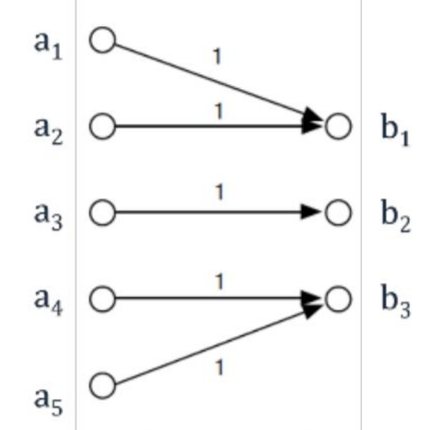
\includegraphics[scale=0.2]{img/determ.png}
    \caption{Grafo di un canale deterministico.}
\end{figure}
\end{minipage}
\begin{minipage}{0.45\textwidth}
\begin{equation*}
    \mathcal{P} = \begin{bmatrix}
    1 & 0 & 0 \\
    1 & 0 & 0 \\
    0 & 1 & 0 \\
    0 & 0 & 1 \\
    0 & 0 & 1 \\
    \end{bmatrix}
\end{equation*}
\end{minipage}
\end{mybox}
Se un solo elemento per riga $i$ \`e uguale a $1$ allora quel valore $a_i$ pu\`o essere ottenuto solo con un possibile $b_j$. Nel canale deterministico infatti conoscere l’ingresso vuol dire conoscere l’uscita, il che implica $H(B|A) = 0$. Poich\`e quindi l’incertezza che rimane su $B$ conoscendo $A$ è nulla si ha 
\begin{equation*}
    I(A;B) = I(B;A) = H(B) - H(B|A) = H(B) = \sum_{b \in B} p(b) \log \info{b}
\end{equation*}
da cui, similmente al caso precedente
\begin{equation}
    \mathcal{C} = \max_{p(a)} I(A;B) = \max_{p(a)} \sum_{b \in B} p(b) \info{b} = \log |B|
\end{equation}
In questo caso, infine, l’equivocazione di canale è data da $H(A|B) = H(A) - H(B)$.

\subsubsection{Canale completamente ceterministico}
Un canale si dice \textbf{completamente deterministico} (corrispondenza uno ad uno) se è sia noiseless che deterministico. In questo caso quindi sia il mittente che il destinatario sanno cosa \`e stato ricevuto/inviato. Alfabeto di ingresso e di uscita
hanno quindi la stessa dimensione, dovendo essere il canale biettivo.
\begin{mybox}{green}{\textit{\textbf{Esempio 4} : \textbf{Canale completamente deterministico}}}
\begin{minipage}{0.45\textwidth}
\begin{figure}[H]
    \centering
    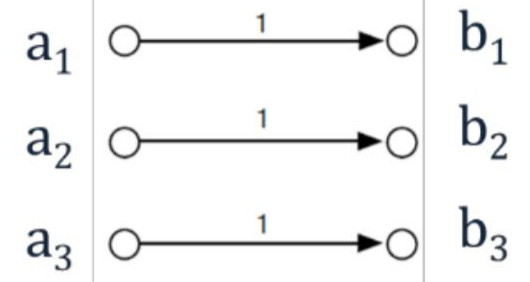
\includegraphics[scale=0.2]{img/cdet.png}
    \caption{Grafo di un canale completamente deterministico.}
\end{figure}
\end{minipage}
\begin{minipage}{0.45\textwidth}
\begin{equation*}
    \mathcal{P} = \begin{bmatrix}
    1 & 0 & 0 \\
    0 & 1 & 0 \\
    0 & 0 & 1 \\
    \end{bmatrix}
\end{equation*}
\end{minipage}
\end{mybox}
Si ha quindi $I(A;B) = H(A) = H(B)$ da cui 
\begin{equation}
    \mathcal{C} = \log r = \log s
\end{equation}

\subsubsection{Canale inutile}
Un canale di definisce \textbf{inutile} se le uscite sono indipendenti dagli ingressi: $p(b|a) = p(b)$. Il destinatario non può derivare alcuna informazione dalla comunicazione, che è stata appunto inutile. Le colonne sono composte da elementi uguali, per cui tutte le righe sono identiche. L'uscita non dipende quindi dall'ingresso.
\begin{mybox}{green}{\textit{\textbf{Esempio 5} : \textbf{Canale inutile}}}
\begin{minipage}{0.45\textwidth}
\begin{figure}[H]
    \centering
    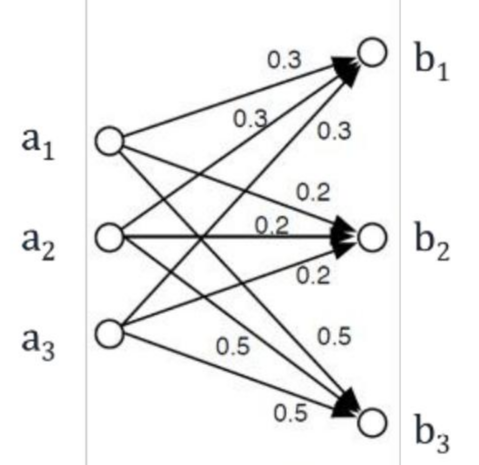
\includegraphics[scale=0.2]{img/inutile.png}
    \caption{Grafo di un canale inutile.}
\end{figure}
\end{minipage}
\begin{minipage}{0.45\textwidth}
\begin{equation*}
    \mathcal{P} = \begin{bmatrix}
    0.3 & 0.2 & 0.5 \\
    0.3 & 0.2 & 0.5 \\
    0.3 & 0.2 & 0.5    
    \end{bmatrix}
\end{equation*}
\end{minipage}
\end{mybox}
Si ha quindi che
\begin{align*}
    H(B|A) &= \sum_{b \in B} \sum_{a \in A} p(a,b) \info{b|a} = \sum_{b \in B} \sum_{a \in A} p(b|a) p(a) \info{b} = \\
    &= \underbrace{\sum_{a \in A} p(a)}_{=1} \sum_{b \in B} \underbrace{p(b|a)}_{=p(b)} \info{b} = \sum_{b \in B} p(b) \info{b} = H(B)
\end{align*}
da cui
\begin{equation*}
    I(A;B) = I(B;A) = H(B) - H(B|A) = H(B) - H(B) = 0
\end{equation*}
e quindi
\begin{equation}
    \mathcal{C} = \max_{p(a)} I(A;B) = 0
\end{equation}

\subsubsection{Canale simmetrico e Canale simmetrico binario}
Un canale di definisce \textbf{simmetrico} se la sua matrice di canale è caratterizzata da righe e colonne che sono
permutazioni degli stessi numeri. Ad esempio:
\begin{equation*}
    \mathcal{P} = \begin{bmatrix}
    0.3 & 0.2 & 0.5 \\
    0.2 & 0.5 & 0.3 \\
    0.5 & 0.3 & 0.2    
    \end{bmatrix}
\end{equation*}
In questo caso si ha che $H(B|A)$ \`e indipendente dalla sorgente ma dipende unicamente dalla matrice $\mathcal{P}$. Dal momento che ogni riga contiene gli stessi valori, indicando con $k$ una costante, si ha che vale
\begin{equation}
    \sum_{j=1}^s p(b_j|a_i) \info{b_j|a_i} = k
\end{equation}
rendendo questa quantit\`a invariante rispetto alla riga (valendo $\forall i = 1, \dots, r$). Si ha quindi che
\begin{align*}
    H(B|A) &= \sum_{b \in B} \sum_{a \in A} p(a,b) \info{b|a} = \sum_{b \in B} \sum_{a \in A} p(b|a)p(a) \info{b|a} = \\
    &= \sum_{a \in A} p(a) \underbrace{\sum_{b \in B} p(b|a) \info{b|a}}_{=k} = k \sum_{a \in A} p(a) = k
\end{align*}
da cui
\begin{equation*}
    I(A;B) = I(B;A) = H(B) - H(B|A) = H(B) - k
\end{equation*}
ovvero che l’informazione mutua dipende da sia da $H(B)$ che dalla matrice di canale e l’unico modo per avere la massima $I(A;B)$ è massimizzare $H(B)$, il che vuol dire avere simboli equiprobabili. \textit{In un canale simmetrico per\`o si hanno simboli in uscita equiprobabili se i simboli in ingresso sono equiprobabili}. Infatti se $p(a) = 1/r$ vale 
\begin{equation}
    p(b) = \sum_{a \in A} p(a,b) = \sum_{a \in A} p(b|a)p(a) = \frac{1}{r} \sum_{a \in A} p(b|a) = \frac{col}{r} = \frac{1}{s}
\end{equation}
dove $col$ rappresenta la somma degli elementi di una colonna della matrice (tutte le colonne sommano a $col$ per definizione).

\begin{mybox}[breakable]{green}{}
Prendiamo ad esempio un canale debolmente simmetrico (un canale si dice debolmente simmetrico quando ogni riga \`e una permutazione di ogni altra riga e le colonne sommano allo stesso valore $col$) di questo tipo
\begin{equation*}
    \mathcal{P} = \begin{bmatrix}
    1/3 & 1/6 & 1/2 \\
    1/3 & 1/2 & 1/6
    \end{bmatrix}
\end{equation*}
Se imponiamo $\forall a \in A$, $p(a) = 1/2$ si ha $p(b) = \frac{1}{2} \times \frac{2}{3} = \frac{1}{3}, \forall b \in B$.
\end{mybox}

In generale si ha quindi che la capacità di un canale simmetrico è
\begin{equation}
    \mathcal{C} = \log(s) - k
\end{equation}

Il \textbf{canale simmetrico binario} (BSC) è un particolare canale simmetrico composto da due simboli in ingresso e da due simboli in uscita $A = B = \{0,1\}$ in cui si ha che $p$ rappresenta la probabilità che ci sia un errore di trasmissione. Si ha quindi che $Pr\{B=1|A=0\} = p = Pr\{B=0|A=1\}$ e $Pr\{B=1|A=1\} = 1-p = Pr\{B=0|A=0\}$:

\begin{minipage}{0.45\textwidth}
\begin{figure}[H]
    \centering
    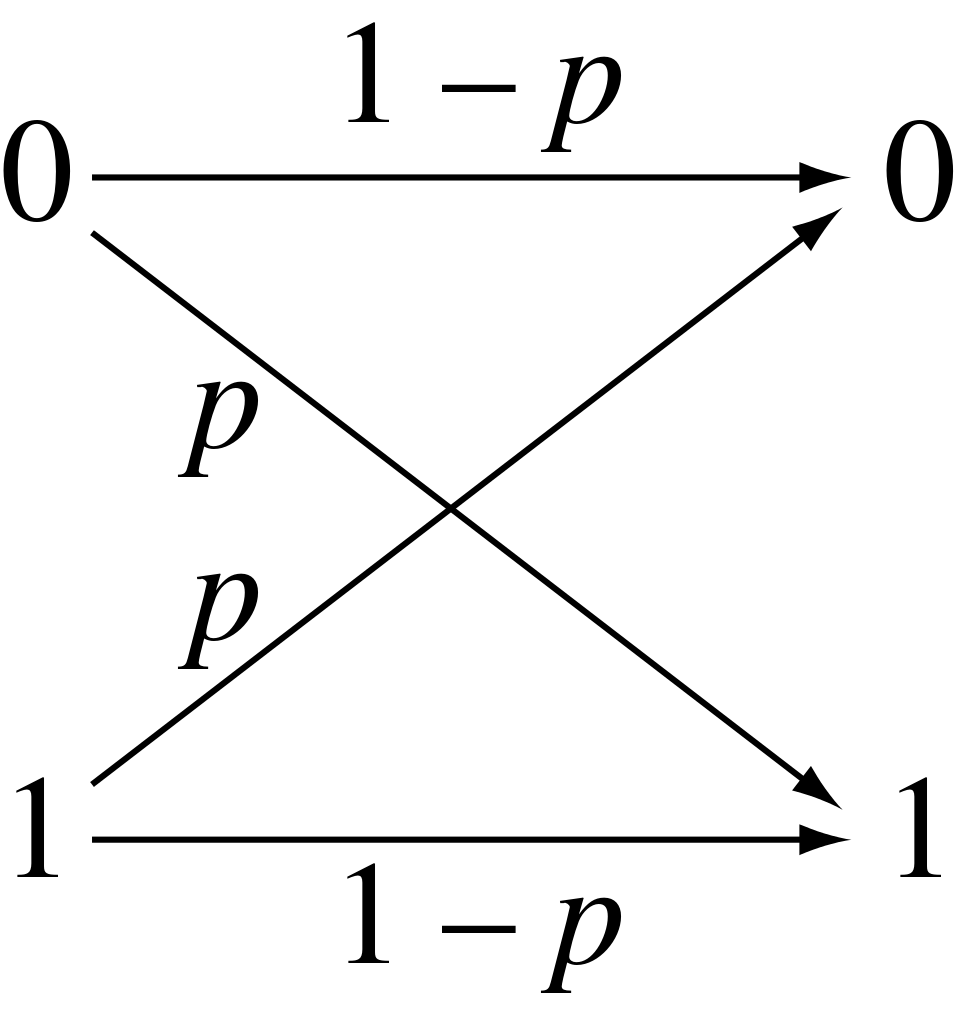
\includegraphics[scale=0.08]{img/bsc.png}
    \caption{Grafo di un canale simmetrico binario.}
\end{figure}
\end{minipage}
\begin{minipage}{0.45\textwidth}
\begin{equation*}
    \mathcal{P} = \begin{bmatrix}
    1-p & p \\
    p & 1-p \\
    \end{bmatrix}
\end{equation*}
\end{minipage}

Verifichiamo che una probabilit\`a uniforme in ingresso implica una probabilit\`a uniforme in uscita:
\begin{align*}
    Pr\{B=0\} &= Pr\{B=0|A=0\}Pr\{A=0\} + Pr\{B=0|A=1\}Pr\{A=1\} = \\
    &= (1-p)Pr\{A=0\} + pPr\{A=1\} \\
    Pr\{B=1\} &= Pr\{B=1|A=0\}Pr\{A=0\} + Pr\{B=1|A=1\}Pr\{A=1\} = \\
    &= pPr\{A=0\} + (1-p)Pr\{A=1\} \\
    \text{Quindi }Pr\{&A=0\} = Pr\{A=1\} = \frac{1}{2} \implies Pr\{B=0\} = Pr\{B=1\} = \frac{1}{2}
\end{align*}
Il BSC \`e il modello più semplice di canale con errori, tuttavia riesce a rappresentare bene la complessità del problema.
\begin{align*}
    I(A;B) &= H(B) - H(B|A) = H(B) - \sum_{a \in A}p(a) H(B|a) = \\
    & \overset{\rho}{=} H(B) - \sum_{a \in A} p(a) H(p) = H(B) - H(p) \leq 1 - H(p)
\end{align*}
Dove l'ultima disuguaglianza vale perch\`e $H(B) \leq 1$ e $H(p)$ \`e l'entropia di una sorgente binaria con probabilit\`a $p$:
\begin{equation*}
    H(p) = p \log \frac{1}{p} + (1-p) \log \frac{1}{1-p}
\end{equation*}
mentre l'uguaglianza $\rho$ vale perch\`e, chiamando 
\begin{itemize}
    \item $p(b_0) \coloneqq Pr\{B=0\}$
    \item $p(b_0|a_0) \coloneqq Pr\{B=0|A=0\} = 1-p $ 
    \item $p(a_1) \coloneqq Pr\{A=1\}$
    \item $\dots$
\end{itemize} si ha
\begin{align*}
&H(B|A) = \sum_{a \in A} \sum_{b \in B} p(b|a)p(a)\info{b|a} = p(b_0|a_0)p(a_0)\info{b_0|a_0} + \\
&+p(b_0|a_1)p(a_1)\info{b_0|a_1} + p(b_1|a_0)p(a_0)\info{b_1|a_0} + p(b_1|a_1)p(a_1)\info{b_1|a_1} = \\
&=p(a_0) \Big [p(b_0|a_0)\info{b_0|a_0} + p(b_1|a_0)\info{b_1|a_0} \Big ] + p(a_1) \Big [p(b_0|a_1)\info{b_0|a_1} + p(b_1|a_1)\info{b_1|a_1} \Big ] = \\
&=p(a_0) \Big [(1-p)\log \frac{1}{1-p} + p \log \frac{1}{p} \Big ] + p(a_1) \Big[ p \log \frac{1}{p} + (1-p)\log \frac{1}{1-p}  \Big ] = \\
& \Big [ p(a_0) + p(a_1) \Big ] \Big [ (1-p)\log \frac{1}{1-p} + p \log \frac{1}{p} \Big ] = H(p)
\end{align*}
Ricordando (vedi Fig. \ref{fig:binentropy}) che l'entropia di una sorgente binaria \`e massima quando la probabilit\`a \`e uniforme si ha
\begin{equation}
    \mathcal{C} = \max_{p(a)} I(A;B) = 1 - H(p)
\end{equation}
L'entropia di $B$ \`e massima quando $p(b)$ \`e uniforme, ma ci\`o vuol dire che la $p(a)$ deve essere uniforme. La capacit\`a di canale di un canale binario simmetrico \`e quindi massima quando la probabilit\`a a priori $p(a)$ \`e uniforme.

\subsubsection{Binary Erasure Channel}
Nel \textbf{binary erasure channel} il mittente può inviare due diversi simboli al destinatario. Un simbolo può essere ricevuto correttamente oppure pu\`o essere \textbf{perso} (in questo caso il destinatario riceve uno speciale simbolo \#). Il canale \`e caratterizzato dalla probabilit\`a $p$ che il simbolo venga perso:

\begin{minipage}{0.45\textwidth}
\begin{figure}[H]
    \centering
    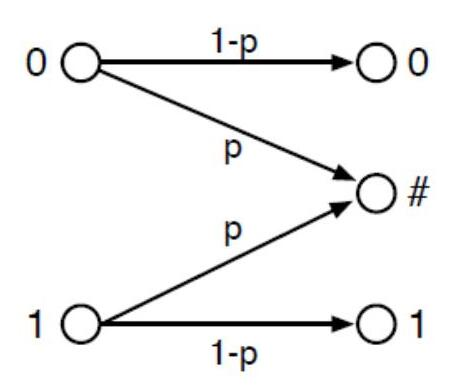
\includegraphics[scale=0.2]{img/erasure.jpg}
    \caption{Grafo di un BEC.}
\end{figure}
\end{minipage}
\begin{minipage}{0.45\textwidth}

\begin{equation*}
    \mathcal{P} = \overbrace{\begin{bmatrix}
    1-p & p & 0 \\
    0 & p & 1-p \\
    \end{bmatrix}}^{0 \hspace{20pt} \# \hspace{20pt} 1}
\end{equation*}
\end{minipage}

Se \`e stato trasmesso $0$ non si può ricevere $1$ e viceversa. Questo modello assume quindi che gli $0$ e $1$ ricevuti vengano ricevuti sempre correttamente e, viceversa, se si \`e ricevuto \# si ha un'ambiguit\`a sul simbolo trasmesso e questa ricezione viene scartata (da qu\`i il nome di BEC). Chiamando $Pr\{A=0\} \coloneqq w, Pr\{A=1\} =1-w$ e avendo che
\begin{itemize}
    \item $Pr\{B=0|A=0\} = Pr\{B=1|A=1\} = 1-p$
    \item $Pr\{B=\#|A=0\} = Pr\{B=\#|A=1\} = p$
    \item $Pr\{B=1|A=0\} = Pr\{B=0|A=1\} = 0$
\end{itemize}
calcoliamo $H(B)$ e $H(B|A)$. Si ha
\begin{align*}
    H(B) &= (1-p)w \log \frac{1}{(1-p)w} + (1-p)(1-w)\log \frac{1}{(1-p)(1-w)} + p \log \frac{1}{p} = \\
    &= (1-p) \Big [ w \log \frac{1}{(1-p)w} + (1-w)\log \frac{1}{(1-p)(1-w)} \Big] + p \log \frac{1}{p} = \\
    &=(1-p) \Big [ w \log \frac{1}{1-p} + w \log \frac{1}{w} + (1-w)\log \frac{1}{1-p} + (1-w)\log \frac{1}{1-w} \Big ] + p \log \frac{1}{p} = \\
    &=(1-p) \Big [ \log \frac{1}{1-p} + H(w) \Big] + p \log \frac{1}{p} =H(p) + (1-p)H(w)
\end{align*}.
\begin{align*}
    H(B|A) &= \sum_{a\in A} \sum_{b \in B} p(b|a)p(a) \log \frac{1}{p(b|a)} = \\
    &= w \Big [(1-p) \log \frac{1}{1-p} + p \log \frac{1}{p} + 0 \Big ] + (1-w) \Big [0 + p \log \frac{1}{p} + (1-p) \log \frac{1}{1-p} \Big ] = \\
    &= w H(p) + (1-w)H(p) = H(p)
\end{align*}
Quindi si ha
\begin{equation*}
    I(A;B) = H(B) - H(B|A) = H(p) + (1-p)H(w) - H(p) = (1-p)H(w)
\end{equation*}
da cui
\begin{equation}
    \mathcal{C} = \max_{p(a)} I(A;B) = \max_{w} (1-p)H(w) = 1-p
\end{equation}
\subsection{Canali in cascata}
\begin{figure}[H]
    \centering
    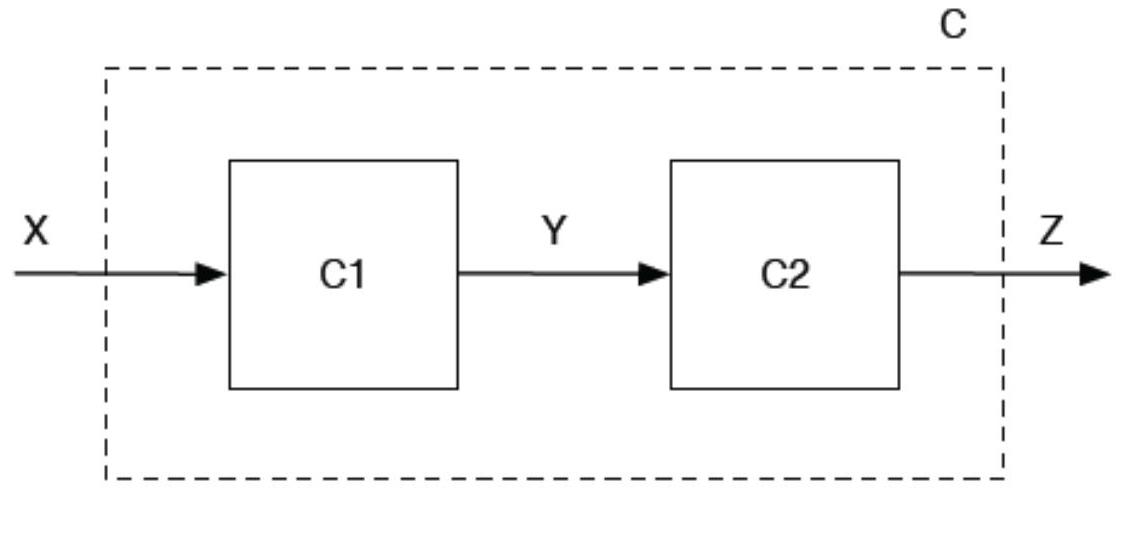
\includegraphics[scale=0.2]{img/cascata.jpg}
    \caption{Due canali in cascata $C_1$ e $C_2$.}
\end{figure}
Due canali $C_1$ e $C_2$ possono essere posti in \textit{cascata}, ovvero uno di seguito all'altro. La matrice di
canale che si ottiene ponendo in cascata due canali $C_1, C_2$ è il prodotto delle matrici di canale dei due canali, ovvero
\begin{equation}
    \mathcal{P}_c = \mathcal{P}_1 \mathcal{P}_2
\end{equation}
Si può verificare che per i canali in cascata l'informazione mutua, man mano che si attraversano i canali, non può aumentare: ad ogni passaggio si può \textbf{solo perdere} informazione e mai guadagnarne:
\begin{equation*}
    \begin{cases}
    H(X|Z) \geq H(X|Y) \implies I(X;Z) \leq I(X;Y)\\
    H(X|Z) \geq H(Y|Z) \implies I(X;Z) \leq I(Y;Z)
    \end{cases}
\end{equation*}
\begin{mybox}{green}{\textbf{\textit{Esempio 6: BSC in cascata}}}
Siano $C_1$ e $C_2$ due BSC in cascata con matrici di canale
\begin{equation*}
    \mathcal{P}_1 = \begin{bmatrix}
    1-p_1 & p_1 \\
    p_1 & 1-p_1
    \end{bmatrix}, \quad 
    \mathcal{P}_2 = \begin{bmatrix}
    1-p_2 & p_2 \\
    p_2 & 1-p_2
    \end{bmatrix}
\end{equation*}
Allora si ha che la matrice di canale risultante \`e data da
\begin{equation*}
    \mathcal{P}_c = \mathcal{P}_1 \mathcal{P}_2 = \begin{bmatrix}
    (1-p_1)(1-p_2) + p_1p_2 & (1-p_1)p_2 + (1-p_2)p_1 \\
    (1-p_1)p_2 + (1-p_2)p_1 & (1-p_1)(1-p_2) + p_1p_2
    \end{bmatrix}
\end{equation*}
da cui, se $p_1 = p_2 = p$ e $(1-p_1)=(1-p_2) = \bar{p}$ si ha
\begin{equation*}
    \mathcal{P}_c = \begin{bmatrix}
    p^2 + \bar{p}^2 & 2 p \bar{p} \\
    2 p \bar{p} & p^2 + \bar{p}^2
    \end{bmatrix}
\end{equation*}
Le due capacit\`a dei singoli tratti valgono quindi
\begin{equation*}
    \mathcal{C}_1 = \mathcal{C}_2 = 1 - H(p)
\end{equation*}
mentre la capacit\`a del canale in cascata \`e
\begin{equation*}
    \mathcal{C}_c = 1 - H(2p\bar{p}) \leq \mathcal{C}_1 = \mathcal{C}_2
\end{equation*}
\end{mybox}
\subsection{Probabilit\`a di Errore e Regola di Decisione}
Se il canale introduce rumore, $H(A|B) \neq 0$, ciò che arriva:
\begin{itemize}
    \item Può essere uguale a quello trasmesso con una certa probabilità.
    \item Può essere diverso da quello trasmesso con un’altra probabilità.
\end{itemize}
quindi il sistema è caratterizzato ovviamente da una certa probabilità di errore.

\textit{Il secondo teorema di Shannon vuole determinare la quantità di informazione che, con una probabiltà di errore piccola a piacere, può attraversare il canale ed essere ricevuta correttamente}. 

C'è quindi innanzitutto bisogno di una regola di decisione che consenta di passare dai simboli ricevuti a quelli inviati. Questa \`e di fondamentale importanza dal momento che, in generale, si ha a che fare con canali “continui” e non discreti, in cui l’alfabeto di uscita può assumere infiniti valori.
\begin{figure}[H]
    \centering
    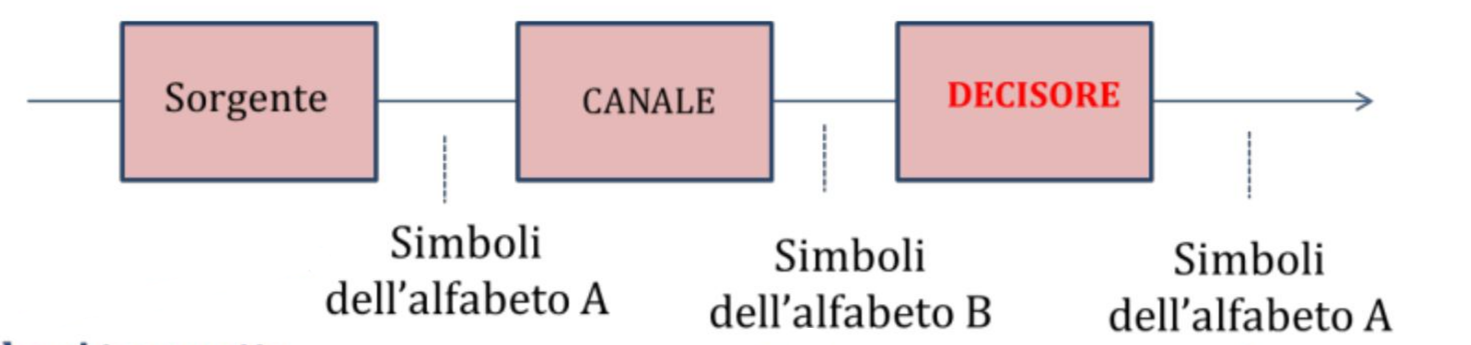
\includegraphics[scale=0.2]{img/decis.png}
\end{figure}
\defn{\textit{Regola di decisione:}} Dato un alfabeto in ingresso $A = \{a_1, \dots, a_r\}$ e uno di uscita $B = \{b_1, \dots, b_s\}$ una regola di decisione \`e una funzione $d:B \to A$ tale che 
\begin{equation}
    \forall b \in B \quad  \exists ! \hspace{4pt}  \hat{a} \in A : d(b) = \hat{a}
\end{equation}
\begin{mybox}{green}{\textbf{\textit{Esempio 7 : Regola di decisione per BSC}}}
Se si ha un BSC con matrice di canale
\begin{equation*}
    \mathcal{P} = \begin{bmatrix}
    0.9 & 0.1
    0.1 & 0.9
    \end{bmatrix}
\end{equation*}
si pu\`o decidere in due modi
\begin{equation*}
    \begin{cases}
    d(0) = 0 \land d(1) = 1 \\
    d(0) = 1 \land d(1) = 0
    \end{cases}
\end{equation*}
La prima regola di decisione non assicura l'assenza di errori ma, mediamente, sbaglier\`a solo nel 10\% dei casi. L'altra regola invece porta a una media del 90\% di errore.
\end{mybox}
In generale si ha che, per un canale con $r$ ingressi ed $s$ uscite, si possono avere $r^s$ regole di decisione. Ad ogni regola di decisione \`e associata un'incertezza ed il nostro obiettivo \`e determinare la migliore regola di decisione. La probabilit\`a di errore media $P_e$ \`e quindi associata ad una certa regola di decisione, in particolare, data una certa regola di decisione $d$, essa pu\`o essere scritta come
\begin{equation}
    P_e \coloneqq \sum_{b \in B} \underset{a \neq \hat{a}}{\sum_{a \in A}} p(a,b) = \sum_{b \in B} \underset{a \neq \hat{a}}{\sum_{a \in A}} p(b|a) p(a) = 1 - \underbrace{\sum_{b \in B} p(b|\hat{a})p (\hat{a})}_{=P_c}
\end{equation}
Dove $P_c$ indica la probabilit\`a di corretta decisione. Come si minimizza questa probabilit\`a? La regola di decisione ottima \`e data dal criterio di \textbf{massima verosimiglianza}:
\begin{align*}
    \min_{d(b)} P_e &= \min_{d(b)} 1 - P_c = \max_{d(b)} P_c = \max_{d(b)} \sum_{b \in B} p(b|\hat{a})p (\hat{a})\\
    &\text{ovvero } \min_{d(b)} p(b|\hat{a})p (\hat{a}), \quad \forall b \in B
\end{align*}
Il simbolo $\hat{a}$ viene quindi scelto come quello che massimizza la probabilità di aver ricevuto il simbolo $b$ condizionata alla trasmissione di $a$:
\begin{equation}
    d(b) = \hat{a} \iff p(b|\hat{a}) p(\hat{a}) \geq p(b|a) p(a), \hspace{10pt} \forall a\in A, b\in B
\end{equation}
che, nel caso di simboli equiprobabili\footnote{Se non si conosce la statistica della sorgente si applica il criterio ML considerando simboli equiprobabili. In questo caso si ottiene una regola di decisione sub-ottima.}, diventa
\begin{equation}
   d(b) = \hat{a} \iff p(b|\hat{a}) \geq p(b|a), \hspace{10pt} \forall a\in A, b\in B
\end{equation}
\subsection{Disuguaglianza di Fano}
Supponiamo, osservando una variabile aleatoria $B$, di voler stimare il valore assunto da un'altra variabile aleatoria $A$ correlata a $B$. La disuguaglianza di Fano connette la probabilit\`a di errore di indovinare il valore di $A$ con l'entropia condizionata $H(A|B)$. L'idea \`e che ci aspettiamo di poter stimare $A$ con una bassa probabilit\`a di errore solo se la probabilit\`a condizionata $H(A|B)$ \`e \textit{piccola}.

Indicando con $P_e$ la probabilit\`a di errore\footnote{In generale $P_e$ pu\`e essere dato da qualunque stimatore $g(B) = \hat{A}$: $P_e = Pr \{\hat{A} \neq A\}$.} si ha la che 
\begin{equation}
\label{eqn:fano}
    H(A|B) \leq H(P_e) + P_e\log (r-1)
\end{equation}
Il membro a destra \`e dato dalla somma di due contributi. Una volta osservato $B$ infatti:
\begin{itemize}
    \item Non si pu\`o determinare se il simbolo ricevuto è affetto da errore o no, e questo \`e il contributo dato da $H(P_e)$, quest'ultima infatti \`e la quantità di informazione di una sorgente binaria con simboli $\{errore, non$ $errore \}$, quindi la quantità di informazione necessaria all'osservatore per dire se c’è stato un errore.
    \item Se c’è errore, con probabilità $P_e$, non si pu\`o determinare quale dei restanti $r-1$ simboli si \`e sbagliato a stimare. Essendo una probabilit\`a condizionata si ha che il valore massimo che può assumere è quello di una sorgente senza condizionamento con $r-1$ simboli tutti equiprobabili, la cui incertezza \`e $\log (r-1)$ pesata per $P_e$. 
\end{itemize}
Ricordando che $r = |A|$ la disuguaglianza di Fano ci dice che l'entropia condizionata \`e massima per $P_e = 1 - \frac{1}{r}$ e vale $H(A|B) = \log r$. Questo avviene quindi quando la probabilit\`a di corretta decisione \`e uniforme sull'insieme $A$, ovvero quando $P_c = \frac{1}{r}$.

\begin{figure}[H]
    \centering
    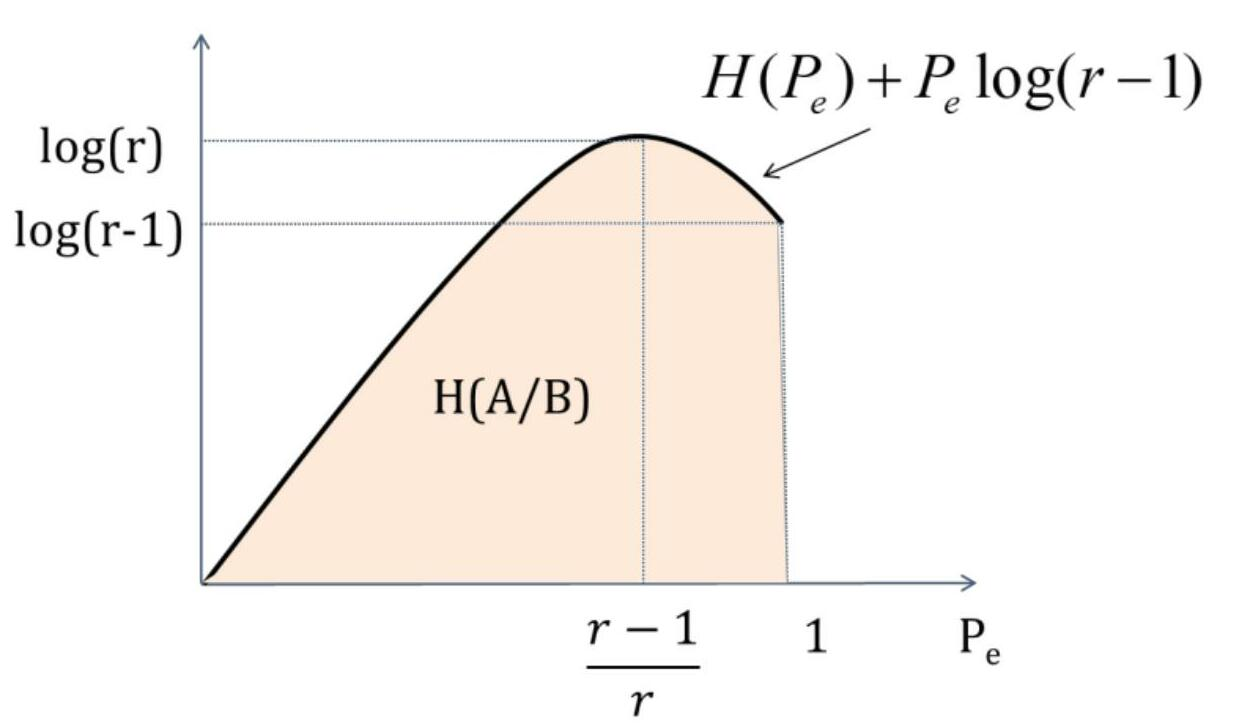
\includegraphics[scale=0.2]{img/fano.jpg}
    \caption{Rappresentazione grafica della disuguaglianza di Fano.}
\end{figure}
Si ha infatti che la funzione $H(P_e) + \log (r-1)$ \`e concava nell'intervallo $P_e \in [0, 1]$, quindi il massimo si ottiene in
\begin{align*}
    \frac{\partial}{\partial P_e} \Big \{ H(P_e) + P_e\log (r-1) \Big \} &= \frac{\partial}{\partial P_e} \Big \{ P_e \log \frac {1}{P_e} + (1-P_e) \log \frac{1}{1 - P_e} + P_e \log(r-1) \Big \} = \\
    &=\log \frac{1}{P_e} - \log \frac{1}{1-P_e} + \log (r-1) = \\
    &=\log \frac{(1-P_e)(r-1)}{P_e} = 0 \implies \frac{(1-P_e)(r-1)}{P_e} = 1 \\
    &\implies P_e = 1 - \frac{1}{r} = \frac{r-1}{r}
\end{align*}
\newline
Vediamo ora la dimostrazione della disuguaglianza di Fano data nella (\ref{eqn:fano}). Questa non \`e l'unica forma in cui si pu\`o presentare ma \`e la forma che pi\`u rapidamente ci permette di mostrare come questa fornisca un limite inferiore alla probabilità d'errore.
\begin{tcolorbox}[enhanced, breakable, frame hidden]
\textbf{Dim}: Proviamo che $H(A|B) - H(P_e) - P_e \log(r-1) \leq 0$. Scriviamo i due termini di entropia in funzione di $P_e$:
\begin{align*}
    H(P_e) + P_e \log (r-1) &= P_e \log \frac{1}{P_e} + P_c \log \frac{1}{P_c} + P_e \log (r-1) = P_e \log \frac{r-1}{P_e} + P_c \log \frac {1}{P_c} = \\
    &=\sum_{b \in B} \underset{a \neq \hat{a}}{\sum_{a \in A}} p(a,b) \log \frac{r-1}{P_e} + \sum_{b \in B} p(\hat{a},b) \log \frac{1}{P_c}
\end{align*}
\begin{align*}
    \hspace{-30pt}H(A|B) &= \sum_{a \in A} \sum_{b \in B} p(a,b) \info{a|b} = \underset{a \neq \hat{a}}{\sum_{a \in A}} \sum_{b \in B} p(a,b) \info{a|b} + \sum_{b \in B} p(\hat{a},b) \info{\hat{a}|b}
\end{align*}
da cui, facendo la differenza, si ha
\begin{align*}
&H(A|B) - H(P_e) + P_e \log (r-1) = \\
&= \underset{a \neq \hat{a}}{\sum_{a \in A}}\sum_{b\in B} p(a,b) \info{a|b} + \sum_{b \in B} p(\hat{a},b) \info{\hat{a}|b} - \sum_{b \in B} \underset{a \neq \hat{a}}{\sum_{a \in A}}  p(a,b) \log \frac{r-1}{P_e} - \sum_{b \in B} p(\hat{a},b) \log \frac{1}{P_c} \\
&=\underset{a \neq \hat{a}}{\sum_{a \in A}}\sum_{b\in B}  p(a,b) \log \frac{P_e}{p(a|b)(r-1)} + \sum_{b \in B} p(\hat{a},b) \log \frac{P_c}{p(\hat{a}|b)} = \\
&=\log e \Bigg [ \underset{a \neq \hat{a}}{\sum_{a \in A}}\sum_{b\in B}  p(a,b) \ln \frac{P_e}{p(a|b)(r-1)} + \sum_{b \in B} p(\hat{a},b) \ln \frac{P_c}{p(\hat{a}|b)} \Bigg ] \leq \\
&\leq \log e \Bigg [ \underset{a \neq \hat{a}}{\sum_{a \in A}}\sum_{b\in B}  p(a,b) \Big (\frac{P_e}{p(a|b)(r-1)} - 1 \Big ) + \sum_{b \in B} p(\hat{a},b) \Big ( \frac{P_c}{p(\hat{a}|b)} - 1 \Big ) \Bigg ] = \\
&=\log e \Bigg [ \underset{a \neq \hat{a}}{\sum_{a \in A}}\sum_{b\in B} \Big (   \frac{P_e p(b)}{r-1} - p(a,b) \Big ) + \sum_{b \in B} P_c p(b) - p(\hat{a},b) \Big ) \Bigg ] = \\
&=\log e \Bigg [ \underset{a \neq \hat{a}}{\sum_{a \in A}} \frac{P_e}{r-1} - p(a) + P_c - p(\hat{a}) \Bigg ] = \\
&=\log e \Bigg [ \frac{P_e(r-1)}{r-1} - \big (1 - p(\hat{a}) \big ) + P_c - p(\hat{a}) \Bigg ] = \\
&=\log e \Big [ P_e + P_c - 1\Big ] = 0 \\
&\hspace{400pt}\square
\end{align*}
\end{tcolorbox}

Si ha inoltre che la disuguaglianza vale come uguaglianza quando, $\forall b \in B$
\begin{equation*}
\begin{cases}
\frac{P_e}{p(a|b)(r-1)} = 1, & \forall a \in A \backslash \{\hat{a}\}\\
\frac{P_c}{p(\hat{a}|b)} = 1
\end{cases} \implies 
\begin{cases}
P_e = p(a|b) (r-1), & \forall a \in A \backslash \{\hat{a}\} \\
P_c = p(\hat{a}|b)
\end{cases}
\end{equation*}
ovvero quando, se si trasmette un simbolo $a$, si ha la stessa probabilità di sbagliare con uno qualsiasi degli altri simboli.

Se prendiamo la disuguaglianza di Fano e la relazione che lega informazione mutua ed equivocazione di canale si ha:
\begin{equation*}
    H(A|B) \leq H(P_e) + P_e \log (r-1) \land H(A|B) = H(A) - I(A;B) \geq H(A) - \mathcal{C}
\end{equation*}
da cui
\begin{equation}
    H(A) \leq H(A|B) \leq H(P_e) + P_e \log (r-1) + \mathcal{C}
\end{equation}

\begin{figure}[H]
    \centering
    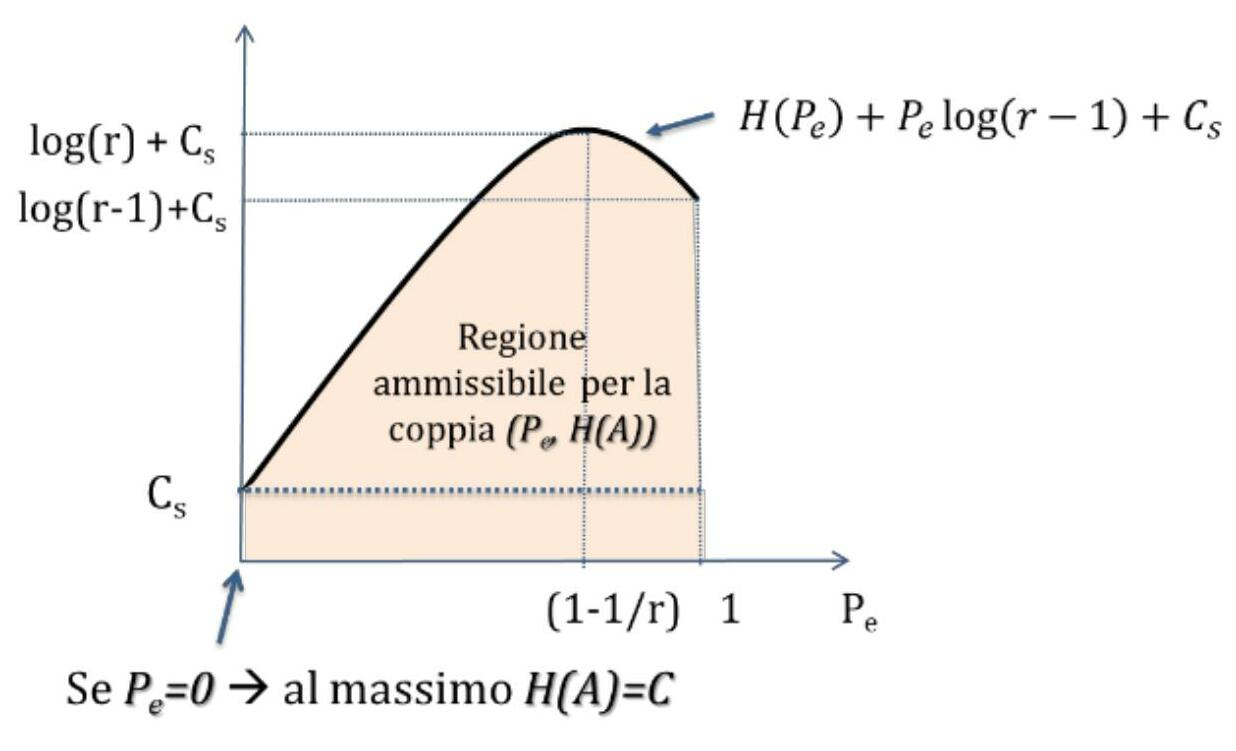
\includegraphics[scale=0.2]{img/equiv.jpg}
    \caption{Regione di di ammissibilit\`a per la coppia $\big ( P_e, H(A) \big )$.}
\end{figure}

Si ha quindi che \textit{se l’entropia della sorgente (il rate) supera la capacit\`a di canale \textbf{\`e impossibile trasmettere con probabilità di errore piccola a piacere}}. Se $H(A) - \mathcal{C} = \tau > 0$ si ha
\begin{equation*}
    H(P_e) + P_e \log (r-1) \geq \tau > 0
\end{equation*}
e quindi un limite inferiore per la $P_e$. Dal momento che esiste questo limite, dato un certo canale con capacità $\mathcal{C}$, vogliamo capire se c`è un modo per rendere la comunicazione più affidabile. \textbf{L’obiettivo è quindi quello di trovare un limite per la quantità di informazione che può essere trasmessa in modo affidabile su un canale rumoroso}. \\
L’affidabilità di una comunicazione può essere migliorata con la codifica di canale, il cui obiettivo consiste proprio nell’aumentare la resistenza dell’informazione al rumore presente sul canale. La codifica di canale \textit{trasforma} la sequenza di dati in ingresso al canale in una nuova sequenza intrinsecamente più robusta agli effetti del rumore. \textit{L’approccio adottato consiste solitamente nell’introdurre ridondanza}. Sfruttando tale ridondanza il decodificatore può ricostruire il messaggio originale anche in presenza di bit errati.
\begin{mybox}{green}{\textit{\textbf{Esempio 6} : \textbf{Codice a ripetizione}}}
Consideriamo un canale simmetrico binario con $p=0.01$ con simboli in ingresso equiprobabili.

\begin{minipage}{0.45\textwidth}
\begin{figure}[H]
    \centering
    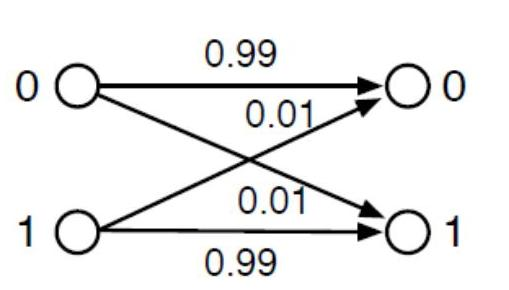
\includegraphics[scale=0.3]{img/bscese.jpg}
\end{figure}
\end{minipage}
\begin{minipage}{0.45\textwidth}
Si ha che 
\begin{equation*}
    \mathcal{P} = \begin{bmatrix}
    0.99 & 0.01 \\
    0.01 & 0.99 \\
    \end{bmatrix}
\end{equation*}
in cui la decisione ottima $d$ \`e data da
\begin{equation*}
    \begin{cases}
    d(0) = 0 \\
    d(1) = 1
    \end{cases} \implies P_e = \frac{0.01 + 0.01}{2} = 0.01
\end{equation*}
\end{minipage}

\vspace{10pt}
Proviamo a migliorare l’affidabilità con una semplice codifica di canale: il \textit{codice a ripetizione}, inviando il $bit$, ad esempio, 3 volte invece di una sola. In sostanza quindi si considera l’estensione di un BSC in cui i simboli che possono essere inviati sul canale sono solamente due $000, 1111$, mentre possono essere ricevute tutte le combinazioni di 3 bit (a seguito degli errori di trasmissione).
\end{mybox}
\begin{mybox}{green}{}
In ricezione la regola di decisione è abbastanza semplice: si sceglie $0$ se sono stati ricevuti più $0$ che $1$, mentre si sceglie $1$ nell'altro caso (avendo preso una ripetizione dispari non si ha mai ambiguità). Poiché la probabilità che $1$ bit venga trasmesso in maniera non corretta e uguale a $p=0.01$ per tutti i simboli, si ha dalla distribuzione binomiale
\begin{align*}
    P_e &= p^2(1-p) \left(
    \begin{array}{c}
      3 \\
      2
    \end{array}
  \right) + p^3(1-p)^0 \left(
    \begin{array}{c}
      3 \\
      3
    \end{array}
  \right) = \\
  &=3p^2(1-p) + p^3 = 3 \times 0.01^2 \times 0.99 + 0.01^3 \approx 3 \cdot 10^{-4}
\end{align*}
L'affidabilità è aumentata a costo di aumentare il numero di bit di ben 3 volte. Possiamo quindi dire che la velocità di trasmissione è ridotta di $1/3$. Se aumentiamo ancora il numero di bit vedremo sempre lo stesso andamento:

\begin{table}[H]
    \centering
    \begin{tabular}{ccc}
    $n$ & $P_e$ & $R$ \\
    \toprule
    $1$ & $10^{-2}$ & $1$ \\
    $3$ & $3$ $\cdot 10^{-4}$ & $1/3$ \\
    $5$ & $3\cdot 10^{-5}$ & $1/5$ \\
    $7$ & $4 \cdot 10^{-7}$ & $1/7$ \\
    $9$ & $10^{-8}$ & $1/8$ \\
    $\vdots$ & $\vdots$ & $\vdots$ \\
    \end{tabular}
    \label{tab:codic}
\end{table}
Quindi se nel tempo di $k$ simboli si trasmette un solo simbolo informativo la velocità di trasmissione si riduce di $k$ volte.
\end{mybox}

\subsection{Canale esteso}
\begin{figure}[H]
    \centering
    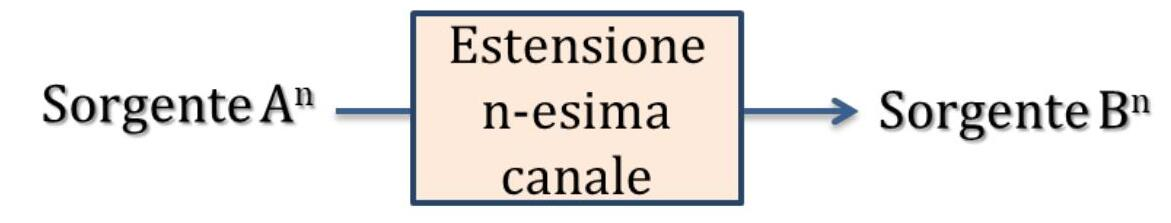
\includegraphics[scale=0.2]{img/estchan.jpg}
\end{figure}
Nell'estensione del canale andiamo a considerare sorgenti estese $A^n, B^n$. Si ha che vale
\begin{align*}
    I(A^n;B^n) \leq n \mathcal{C}
\end{align*}
\begin{tcolorbox}[enhanced, breakable, frame hidden]
\textbf{Dim}:
\begin{align*}
    I(A^n;B^n) &= H(B^n) - H(B^n|A^n) = H(B^n) - \sum_{i=1}^n H(B_i|B_1, \dots, B_{i-1}, A^n) = \\
    &\overset{\eta}{=} H(B^n) - \sum_{i=1}^n H(B_i|A_i) \leq \sum_{i=1}^n H(B_i) - \sum_{i=1}^n H(B_i|A_i) = \sum_{i=1}^n I(A_i; B_i) \leq \\
    &\leq n \mathcal{C} \hspace{350pt} \square
\end{align*}
\end{tcolorbox}
Dove l'uguaglianza $\eta$ vale perche il canale \`e discreto e senza memoria, da cui $B_i$ dipdende unicamente da $A_i$ ed \`e quindi condizionalmente indipendente da tutto il resto. La prima disuguaglianza vale invece dalla (\ref{eqn:leq}) e la seconda dalla definizione di capactit\`a. \\
Si pu\`o estendere la disuguaglianza di Fano all'estensione $n$-esima del canale come
\begin{equation}
    H(A^n|B^n) \leq H(P_e^n) + P_e^n \log (r^n - 1)
\end{equation}
dove $P_e^n$ \`e la probabilit\`a di errore associata a una sequenza di $n$ simboli e \textcolor{red}{non} la potenza $n$-esima della $P_e$ per un simbolo.
Abbiamo visto che aumentando il numero di bit usati per codificare un simbolo della sorgente si riduce la $P_e$ ma anche la velocità con cui si trasmettono i dati. Consideriamo allora un altro esempio: dato lo stesso canale BSC visto sopra, cambiamo codifica, invece di inviare un bit per volta, ne inviamo due e codifichiamo il messaggio fatto da due bit in una parola di codice fatta da tre bit:
 
 \begin{minipage}{0.45\textwidth}
 \begin{figure}[H]
     \centering
     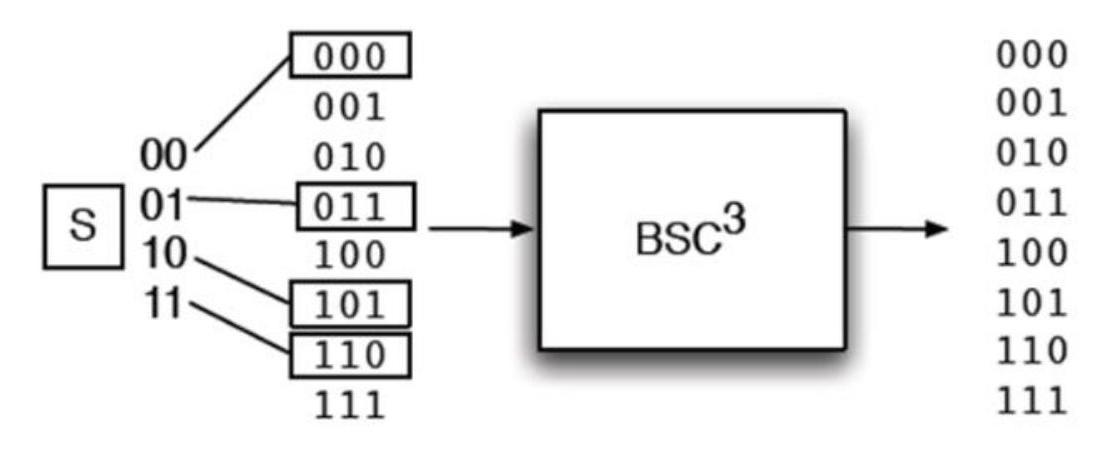
\includegraphics[scale=0.2]{img/bsc3.jpg}
 \end{figure}
 \end{minipage} \hfill
 \begin{minipage}{0.45\textwidth}
 La decisione ottima $d$ \`e data da
\begin{equation*}
    \begin{cases}
    d(000) = d(001) = 00 \\
    d(010) = d(011) = 01 \\
    d(100) = d(101) = 10 \\
    d(110) = d(111) = 11 \\
    \end{cases} \implies P_e \approx 2 \cdot 10^{-2}
\end{equation*}
Con un rate $R=\frac{2}{3}$ dal momento che vengono inviati $3$ bit per rappresentarne $2$.
\end{minipage}

La codifica di canale associa a blocchi di $k$ bit in ingresso blocchi di $n$ bit, con $n \geq k$ il che comporta che il \textbf{coding rate} $R_c$ segua la legge
\begin{equation}
    R_c \coloneqq \frac{k}{n}
\end{equation}
dal momento che, se per ogni parola della sorgente lunga $k$ bit se ne inviano $n$ la velocità di trasmissione si ridurr\`a: se invio $1$ $bit$ ogni $T$ unit\`a di tempo (ad esempio secondi): senza codifica sono necessari $kT$ unit\`a di tempo per terminare la comunicazione, con la codifica sono necessari $nT$ unit\`a di tempo, con $n\geq k$. Abbiamo quindi una struttura di questo tipo:
\begin{figure}[H]
    \centering
    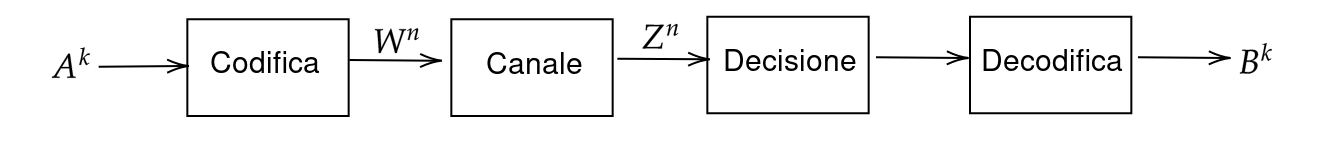
\includegraphics[scale=0.3]{img/diagramma.png}
\end{figure}
In cui, seguendo l'esempio con $k=2, n=3$, potremmo avere $A^2 = \{00, 01, 10, 11\}, W^3 = \{000, 011, 101, 110\}$ e $Z^3 = \{000, 001, 010, 011, 100, 101, 110, 100\}$. In questo sistema si ha che
\begin{itemize}
    \item $H(A^k|B^k) = H(A^k) - I(A^k;B^k)$
    \item Con i canali in cascata: $I(A^k; B^k) \leq I(W^n;Z^n)$
    \item Con un canale esteso: $I(W^n;Z^n) \leq n \mathcal{C}$
\end{itemize}
Questo comporta
\begin{equation*}
    \begin{cases}
    H(A^k|B^k) \geq H(A^k) - n \mathcal{C} = kH(A) - n \mathcal{C} \\
    H(A^k|B^k) \leq H(P_e^n) + P_e^n \log (r^k - 1)
    \end{cases} \implies k H(A) \leq H(P_e^n) + P_e^n \log (r^k -1) + n \mathcal{C}
\end{equation*}
Nel limite in cui $P_e \to 0$ si ha che 
\begin{equation*}
    kH(A) \leq n \mathcal{C} \implies H(A) \leq \frac{n}{k} \mathcal{C} = \frac{\mathcal{C}}{R_c}
\end{equation*}

\begin{minipage}{0.4\textwidth}
quindi deve essere che 
\vspace{15pt}
\begin{mybox}{blue}{}
\vspace{-10pt}
\begin{equation}
    R = R_c H(A) \leq \mathcal{C}
\end{equation}
\end{mybox}
\end{minipage} \hfill
\begin{minipage}{0.4\textwidth}
\begin{figure}[H]
    \centering
    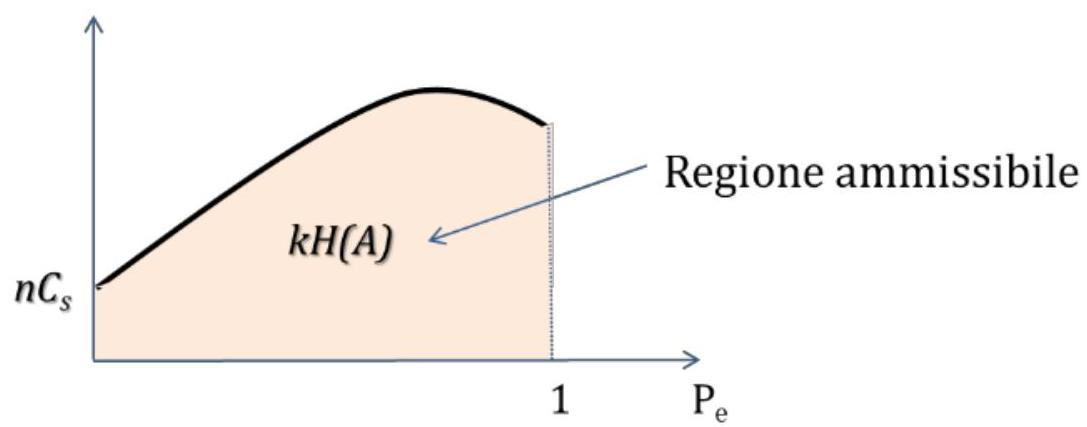
\includegraphics[scale=0.2]{img/ammiss.jpg}
\end{figure}
\end{minipage}

ovvero che, per poter lavorare nella regione $P_e \rightarrow 0$ si deve:
\begin{itemize}
    \item \textbf{Ridurre il rate di trasmissione}:
    \begin{enumerate}
        \item \textit{Riducendo il rate} (entropia) \textit{della sorgente} $A$, quindi comprimendo di pi\`u (non \`e detto che sia possibile).
        \item Ridcuendo $R_c$, ovvero \textit{aumentando la ridondanza della codifica di canale}: fissata $H(A)$ se la sorgente emette un bit ogni $T_s$ unit\`a di tempo, con modulazione binaria la banda necessaria $B$ sarebbe, se $R_c = 1$
        \begin{equation*}
            B \approx \frac{1}{T_s}
        \end{equation*}
        se invece il canale deve far passare $n$ bit in $kT_s$ unit\`a di tempo la banda necessaria sarebbe
        \begin{equation*}
            B \approx \frac{n}{kT_s} = \frac{R_c}{T_s}
        \end{equation*}
        il che implica che \textit{serve una banda maggiore}.
    \end{enumerate}
    \item \textbf{Aumentare la capacità di canale} $\mathcal{C}$ aumentando il \textit{Rapporto Segnale Rumore} sul canale: la $P_e$ si ridurr\`a dal momento che il canale introduce una minore equivocazione.
\end{itemize}
\subsection{Secondo Teorema di Shannon}
Il secondo teorema di Shannon da un’altra possibilità, ci dice che fissato il rate di sorgente e la capacità di canale, si può mantenere costante il rapporto $R_c = \frac{n}{k}$ (ovvero non aumentando la banda) \textbf{incrementando la lunghezza del blocco in ingresso al codificatore}. In sostanza dimostra che \textit{è possibile ridurre arbitrariamente la probabilità di errore, con il vincolo che il rate di trasmissione sia inferiore alla capacita di canale}.

Supponiamo di avere una sorgente discreta senza memoria con alfabeto $A$, entropia $H(A)$ e un canale discreto senza memoria con capacità per simbolo pari a $\mathcal{C}$ $[bit/simbolo]$. Il \textbf{Secondo Teorema di Shannon} afferma che

\textit{Esiste un sistema di codifica con $R_c = \frac{k}{n}$ e $R = R_c H(A) < \mathcal{C}$ che permette la trasmissione dell’informazione emessa dalla sorgente sul canale con una probabilità di errore arbitrariamente piccola.}

Questo pu\`o essere espresso come
\begin{equation}
    \forall \epsilon > 0, \exists n_0 \in \mathbb{N}: \forall n > n_0 \text{ si ha } P_e < \epsilon 
\end{equation}
ed in particolare si pu\`o scrivere, detta $E(\cdot)$ una funzione  convessa decrescente e positiva in $[0,\mathcal{C}]$
\begin{equation}
    P_e < e^{-nE(R_s)} \text{ con }R_s \coloneqq R_c H(A)
\end{equation}

Il Secondo Teorema di Shannon \textit{non fornisce dettagli sul sistema di codifica necessario} per ottenere probabilità d’errore arbitrariamente piccola, ma afferma solo che, \textit{se} $R < \mathcal{C}$, esso \textit{\textbf{esiste}}. Nella pratica, si può verificare che per ridurre la probabilità d’errore si deve incrementare il numero di $bit$ in ingresso al codificatore. Per $n \to \infty$ per\`o il tempo necessario per la trasmissione del messaggio codificato tende all’infinito e la complessità di codifica e decodifica cresce.
\subsection{Canale Gaussiano}
Fino ad ora abbiamo considerato canali discreti. Nella realtà le informazioni vengono inviate in canali analogici e si devono quindi considerare sorgenti analogiche. Studiamo in particolare il canale con rumore bianco gaussiano (\textit{AWGN})\footnote{Questo canale \`e un buon modello per molte comunicazioni, come quella telefonica o quella satellitare.}, che è caratterizzato da un modello a rumore additivo tra ingresso $X$ ed uscita $Y$:
\begin{equation}
    Y = X + Z
\end{equation}
in cui il rumore $Z = \mathcal{N}(0; \sigma_z^2)$ con $X \perp Z$ ($X$ e $Z$ incorrelate). \textit{Data la bianchezza del rumore il canale \`e quindi senza memoria e stazionario}. \\
Anche nel caso di segnali analogici poi vale quanto abbiamo visto, e la capacità è definita come il massimo
dell’informazione mutua:
\begin{align*}
    \mathcal{C} &= \max_{X} I(X;Y) = \max_{X} \big [ h(Y) - h(Y|X) \big ]= \\
    &=\max_{X} \big [ h(Y) - h(X+Z|X) \big ]= \max_{X} \big [ h(Y) - h(Z|X) \big ]= \\
    &=\max_{X} \big [ h(Y) - h(Z) \big ] = \max_{X} \big [ h(Y) - \frac{1}{2}\log (2 \pi \sigma_z^2 e )\big ]
\end{align*}
che si ottiene quando $Y$ \`e gaussiana
\begin{equation*}
    \mathcal{C} = \frac{1}{2}\log (2 \pi \sigma_y^2 e) - \frac{1}{2}\log (2 \pi \sigma_z^2 e) = \frac{1}{2} \log \frac{\sigma_y^2}{\sigma_z^2}
\end{equation*}
ed essendo $X \perp Z$ si ha $\sigma_y^2 = \sigma_x^2 + \sigma_z^2$ da cui
\begin{equation}
    \mathcal{C} = \frac{1}{2} \log \bigg ( 1 + \frac{\sigma_x^2}{\sigma_z^2} \bigg )
\end{equation}

Stiamo per\`o considerando un canale con banda infinita: nella pratica tutti i canali hanno banda limitata $[-B,B]$ e, se non vogliamo avere aliasing, il segnale deve essere campionato\footnote{Per il Teorema del Campionamento di Nyquist-Shannon.} con una frequenza almeno pari a $2B$ campioni$/s$. Ogni campione di segnale ha potenza $P_X = \sigma_x^2$ mentre la potenza del rumore, assumento che la densità spettrale di potenza del segnale sia $\sigma_x^2 = \frac{N_0}{2} \frac{[W]}{[Hz]}$, \`e data da $P_Z = \sigma_z^2 = N_0 B$ da cui
\begin{equation*}
    \mathcal{C} = \frac{1}{2} \log \bigg ( 1 + \frac{\sigma_x^2}{N_0 B} \bigg ) \hspace{10pt} \frac{bit}{\text{trasmissione}}
\end{equation*}
e se teniamo in considerazione la frequenza di campionamento $f = 2B$ possiamo usare il canale $2B$ volte al secondo, quindi
\begin{equation}
    \mathcal{C} = f \frac{1}{2} \log \bigg ( 1 + \frac{\sigma_x^2}{N_0 B} \bigg ) = B \log \bigg ( 1 + \frac{\sigma_x^2}{N_0 B} \bigg ) = B \log \big (1 + SNR \big ) \hspace{5pt} \frac{bit}{s}
\end{equation}
che è famosa formula di Shannon della capacità di un canale \textit{AWGN}. \\
Dalla formula si vede che la capacità dipende dalla banda e dal \textit{SNR}, quindi dalla potenza del segnale in ingresso $P_x$. Aumentando la potenza di trasmissione aumenta il \textit{SNR} e ovviamente aumenta la capacità, ma la crescita è logaritmica. Aumentando la banda $B$ aumenta il termine a moltiplicare ma anche la quantità di rumore che entra nel segnale, quindi si ha un asintoto
\begin{align*}
    \lim_{B \to \infty} \mathcal{C} &= \lim_{B \to \infty} B \log \bigg ( 1 + \frac{\sigma_x^2}{BN_0} \bigg ) = \\
    &=\lim_{B \to \infty} (\log e) B \ln \bigg ( 1 + \frac{\sigma_x^2}{BN_0} \bigg ) \approx \lim_{B \to \infty} (\log e) B \frac{\sigma_x^2}{BN_0} = (\log e) \frac{\sigma_x^2}{N_0}
\end{align*}
dove si \`e usato l’approssimazione al primo ordine $\ln (1 + x) \approx x$ con $x \ll 1$. \`E chiaro quindi che, anche aumentando la banda $B$ non si pu\`o scendere sotto il limite di $\approx 1.44 \sigma_x^2/N_0$.

\subsection{Curva di Shannon}
Introduciamo adesso la curva di Shannon, che mostra l'esistenza di un \textit{trade-off} tra potenza del segnale in ingresso $P_x$ e banda $B$ in ogni sistema di comunicazione. Dal momento che deve essere $R < \mathcal{C}$ si deve avere
\begin{equation}
    R < B \log \bigg ( 1 + \frac{P_x}{N_0 B}\bigg )
\end{equation}
dividendo entrambi i membri per $B$ si ottiene l'\textit{efficienza spettrale} $r \coloneqq R/B$
\begin{equation}
    r < \log \bigg ( 1 + \frac{P_x}{N_0 B} \bigg )
\end{equation}
ovvero il numero di $bits$ per secondo che possono essere trasmessi in un'unit\`a di banda (in 1 $Hz$). Osservando che $P_x = E_b R$, dove $E_b$ \`e l'energia per bit trasmesso, otteniamo
\begin{equation}
\label{eqn:shanncurve}
    r < \log \bigg (1 + r \frac{E_b}{N_0} \bigg )
\end{equation}
Questa relazione definisce le regioni di ammissibilit\`a di efficienza spettrale al variare del rapporto $E_b/N_0$. Il luogo dei punti in cui $r = \log (1 + r E_b/N_0 )$ prende il nome di \textbf{curva di Shannon} (vedi Figura \ref{fig:shcrv}). Quest'ultima divide il piano $(E_b/N_0, r)$ in due parti: la regione sotto la curva (in blu) rappresenta l'insieme dei punti per cui \`e possibile ottenere una comunicazione affidabile (quella sopra in cui non \`e possibile). Per studiare il comportamento del $ENR$ (\textit{Energy-Noise Ratio}) al variare di $r$ eleviamo alla potenza di $2$ entrambi i membri della \ref{eqn:shanncurve}, da cui
\begin{equation}
\frac{2^r - 1}{r} < \frac{E_b}{N_0}
\end{equation}
Possiamo quindi studiare il comportamento asintotico:
    \begin{equation*}
    \begin{cases}
        r \to \infty \implies \frac{E_b}{N_0} \to \infty \\
        r \to 0 \implies \frac{E_b}{N_0} \to \ln 2
    \end{cases}
    \end{equation*}
ovvero che la curva di Shannon ha un asintoto verticale in $E_b/N_0 = \ln 2 \approx 1.6$ $dB$ al di sotto del quale non \`e possibile avere una trasmissione affidabile, per ogni valore di $r$.
\begin{figure}[H]
    \centering
    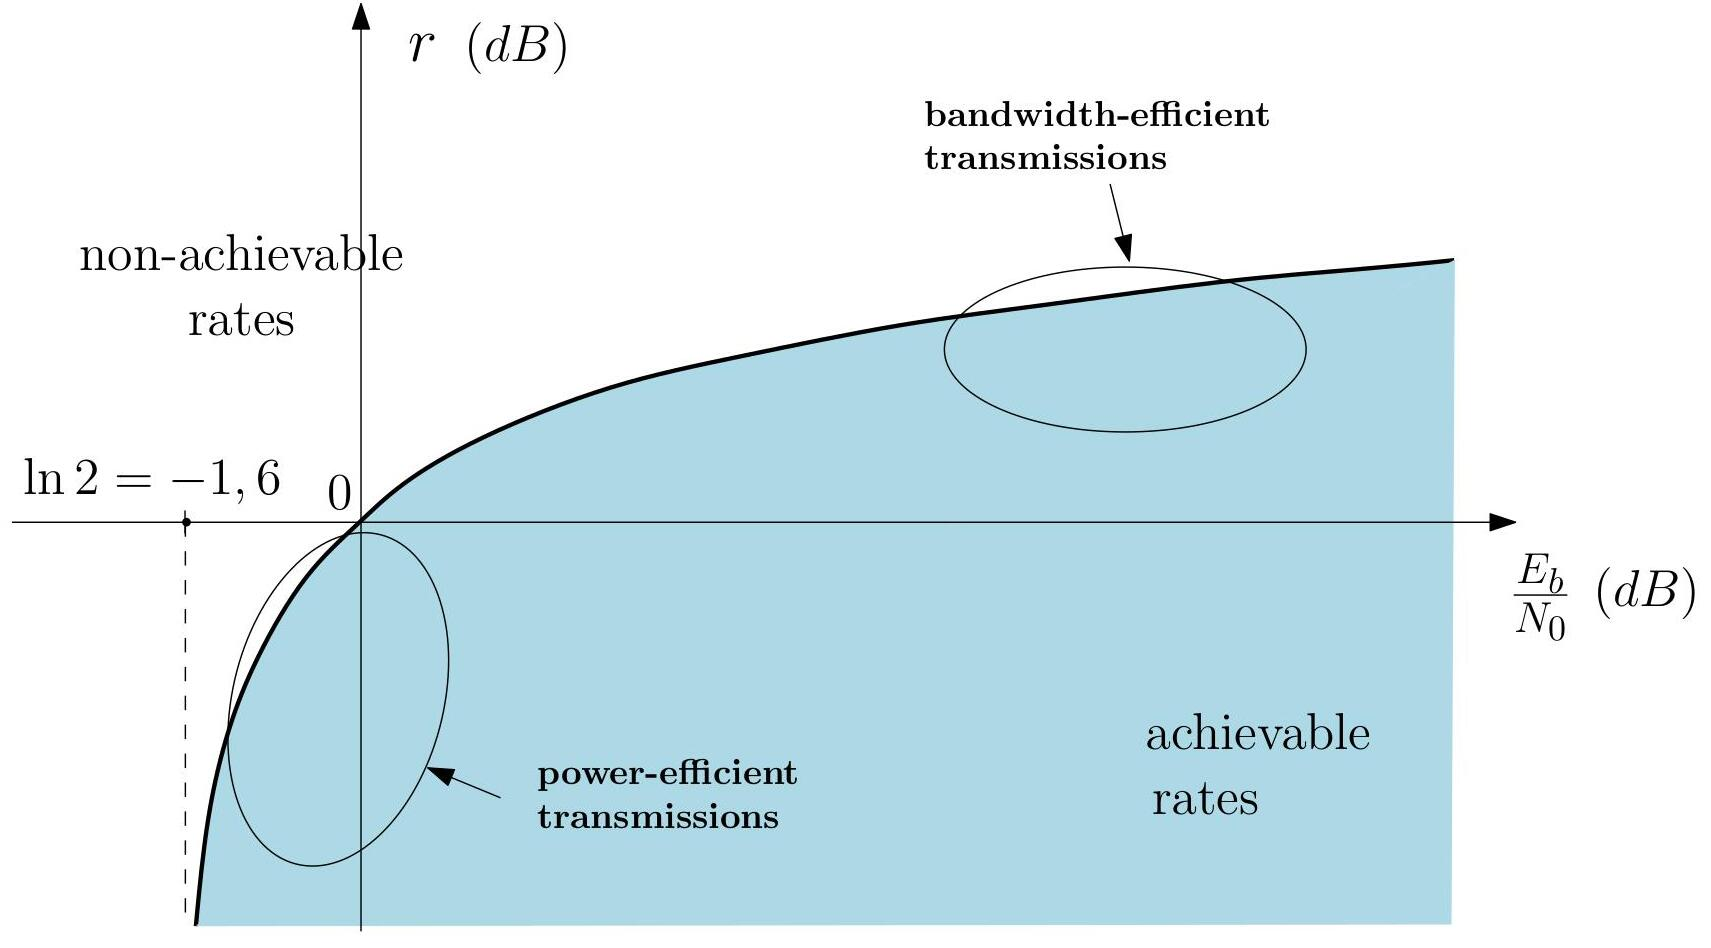
\includegraphics[scale=0.2]{img/shanno.jpg}
    \caption{Curva di capacit\`a di Shannon.}
    \label{fig:shcrv}
\end{figure}
La curva che si ottiene è teorica, ma tali risultati sono molto utili nella progettazione di un sistema reale, in quanto definiscono il \textit{\textbf{limite superiore} delle prestazioni ottenibili da un sistema} modellabile con un canale corrotto da rumore \textit{AWGN}. Nella regione dei punti operativi (raggiungibili) ovviamente più il punto di lavoro reale che si riesce ad ottenere si avvicina alla curva limite $(R=C)$ più il sistema è efficiente. Per le comunicazioni il cui principale limite è la potenza di trasmissione ($r \ll 1$) si hanno trasmissioni efficienti in potenza, mentre per i sistemi dove è la banda ad essere il limite principale ($r \gg 1$) si hanno trasmissioni efficienti in banda.